\section{\heiti{经典方法复现}}
本项目复现多个可以显著提高滤波器性能的硬件算法,如著名的快速傅立叶变换(Fast Fourier Transformation)、Booth
无进位乘法(Booth Multiplication Algorithm)。
\subsection{\heiti{基于 Cooley-Tukey FFT 算法实现的 FIR 滤波器}}

本项目实现了 Cooley-Tukey 的快速傅立叶变换算法(Fast Fourier Transformatioin, FFT)。

实现细节可见算法理论的经典教材算法导论\cite[Chap30]{Cormen2022} 一书。

由第二部分如果采用无优化的离散 Fourier 变换算法在硬件上进行运算,那么完成一次完整的 DFT 需要进行
$\O (n^2)$ 次乘法和 $\O(n^2)$ 次加法。其中 $n$ 代表 DFT 变换器的阶数(或者滤波器的抽头数)。这个速度一般
而言是硬件运算能承受的最大时间复杂度。

在二十世纪六十年代,来自 Princeton 的计算机科学家 Cooley 和数学家 Tukey 发明了一种基于快速幂算法和 Gauss 和算术性质
的快速离散 Fourier 算法。其可以通过数量级地减少 DFT 算法中的乘法次数
大大加快原有离散 Fourier 变换的运算速度。本质上这一算法的理论框架已经被德国数学家 Carl Friedrich Gauss 于 19世纪初
发现并证明,参见\href{https://en.wikipedia.org/wiki/Cooley–Tukey_FFT_algorithm}{Wikipedia}。核心公式即
 $n= 2^m$ 时
\begin{eqnarray*}
    \mathrm{DFT}_{n}(\left\{X_i\right\}_i )_k =  
    \mathrm{DFT}_{\frac{n}{2}}(\left\{X_{2i}\right\}_i )_k + \omega_n^{k} 
    \mathrm{DFT}_{\frac{n}{2}}(\left\{X_{2i+1}\right\}_i )_k,\qquad k=0,..,\frac{n}{2}\\
    \mathrm{DFT}_{n}(\left\{X_i\right\}_i )_{k+\frac{n}{2}} =  
    \mathrm{DFT}_{\frac{n}{2}}(\left\{X_{2i}\right\}_i )_{k+\frac{n}{2}} - \omega_n^{k} 
    \mathrm{DFT}_{\frac{n}{2}}(\left\{X_{2i+1}\right\}_i )_{k+\frac{n}{2}},\qquad k=0,..,\frac{n}{2}\\
    \omega_n = e^{-\frac{2\pi \sqrt{-1}}{n}}
\end{eqnarray*}

于是通过线性变换将 $n$-阶 DFT 转换成 $\frac{n}{2}$-阶 DFT。分治算法复杂度主定理立即得到其理论时间复杂度
能够达到 $\O (n \ln n)$。

这里的实现方式主要参考了算法导论一书的 FFT 章节见 \cite[Polynomials and FFT]{Cormen2022}。

另外我们团队也考虑到了古老的 Wingoard 加速算法(Wingoard Fourier Transformation,WFT)。其主要处理内积加速。

本质和 Karatsuba 加速类似,即对 $m = 2n/2n+1$-维向量内积 $\langle \mathbf{x}, \mathbf{y}\rangle = \sum_{k=1}^{k=2n}x_k y_k$
分治处理,构造
\begin{align*}
    &\qquad\qquad     W(\mathbf{x}) = \sum_{i=1}^{i=n} x_{2i-1} x_{2i}\\
    &\qquad\qquad    \langle \mathbf{x}, \mathbf{y}\rangle =
    \begin{cases}
        \sum_{i=1}^{i=n}(x_{2i-1} + y_{2i})(x_{2i} + y_{2i_1}) - W(\mathbf{x}) - W(\mathbf{y}) \quad& m=2n\\
        \sum_{i=1}^{i=n}(x_{2i-1} + y_{2i})(x_{2i} + y_{2i_1}) - W(\mathbf{x}) - W(\mathbf{y})  + x_n y_n 
        \quad& m=2n+1
    \end{cases} 
\end{align*}
如果在向量中保存 $W(\mathbf{v})$ 的值则得到用上式(Wingoard 加速核心公式)所需的乘法次数大概减半 $\Theta(m) \to \Theta(\frac{m}{2})$。
这在乘法器代价高的硬件框架上较为有用。特别地 Wingoard 算子 $W(-)$ 的更新几乎是常量时间的(单次或两次乘法器运算时间),从而加速的稳定性得到保证。

\subsection{\heiti{冗余计算和 Booth 乘法}}

此处是简单介绍冗余计算的概念。

本质上所有的大整数/高精度浮点数的计算都涉及到进位问题。
原因很简单,在整数的范畴中 $a^2$ 往往要大于 $a$。一个十分聪明的调整办法就是在表示数的时候
不是采用 $[0,N]$ 区间而是 $[-\lfloor\frac{N}{2}\rfloor,\lfloor\frac{N}{2}\rfloor]$。

逆元的产生催生出一种硬件快速乘法:无进位乘法。

Booth 乘法器的原生算法可以在保持设定精度的前提下显著地提升滤波器中乘法器的性能。
后续项目采用的 Booth 乘法是``基四最小冗余(Minimal Redundant Radix-4,mr4)''方案的实现。
具体方式本文放在第三部分阐述。

\subsection{\heiti{基于量化感知的自适应加速}}

这一节本文关注的是此问题的发展前景:利用机器学习方法实现滤波器的各种自适应功能。

\paragraph{\heiti{自适应滤波器的常见场景}}

自适应滤波器是一种参数即时更新滤波技术。

自适应滤波器通过模型训练不断更新参数,使得滤波器的输出更加接近预期的输出。

一般而言,整个系统提供输入波形与预期波形。输入波形传入滤波器,通过相应计算得到输出波形。自适应滤波器旨在通过最小化输出波形与预期波形的某种差距以提高滤波能力。

自适应滤波器大体上可以完成四种任务。

\begin{itemize}
    \item 系统识别

          在实际场景应用中,我们需要识别一些未知的系统,这些系统会影响波形的传递,使得传递波形与原始波形不同。
          自适应滤波器可用于识别一个未知系统。我们将输入波形分别通过滤波器以及未知系统,将未知系统的输出波形作为预期波形,与通过了输入波形的自适应滤波器所输出的波形进行对比,并通过机器学习等方式训练滤波器参数,该滤波器最终可以代表未知系统的近似模型。

          \begin{center}
              \begin{figure}[ht!]
                  \centering
                  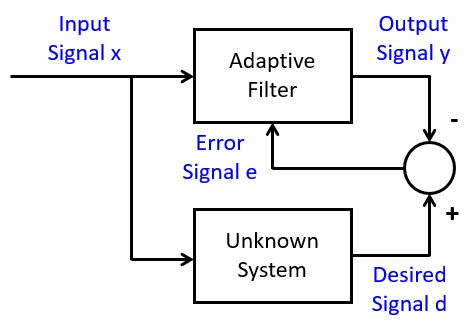
\includegraphics[scale=0.5]{figures/sec2systemid.jpg}
                  \caption{系统识别滤波器工作过程}
                  \label{fig:systemID}
              \end{figure}
          \end{center}

    \item 噪声抵消

          噪声抵消出现于传递波形包含噪声的情形。某一噪声在未知系统影响下被叠加到另外一段波形中,该波形被非线性地叠加在另一端输入波形中。我们希望通过滤波器还原出输入波形的初始形式。
          实际场景中,自适应滤波器将利用初始波形,噪声以及含噪声的最终波形进行参数训练。
          滤波器在噪声抵消的过程中将实际噪声作为输入,通过滤波器后将输出波形叠加到最终波形上,以逼近初始波形。

          \begin{center}
              \begin{figure}[ht!]
                  \centering
                  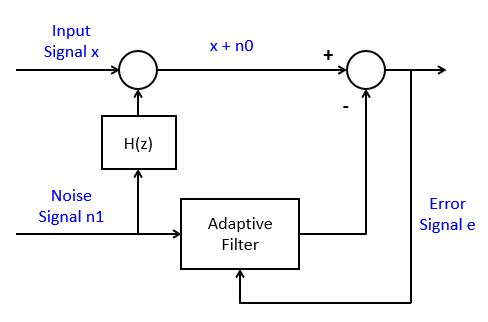
\includegraphics[scale = 0.5]{figures/sec2noisecancellation.jpg}
                  \caption{噪声抵消滤波器工作过程}
                  \label{fig:noisecancellation}
              \end{figure}
          \end{center}

    \item 信号矫正

          在滤波过程中会出现一些信号扭曲的情形,导致收到的信号会与实际信号产生偏离。自适应信号平衡任务即是通过滤波器将发生偏离的信号进行矫正,以使得其逼近实际的无偏差信号。
          \begin{center}
              \begin{figure}[ht!]
                  \centering
                  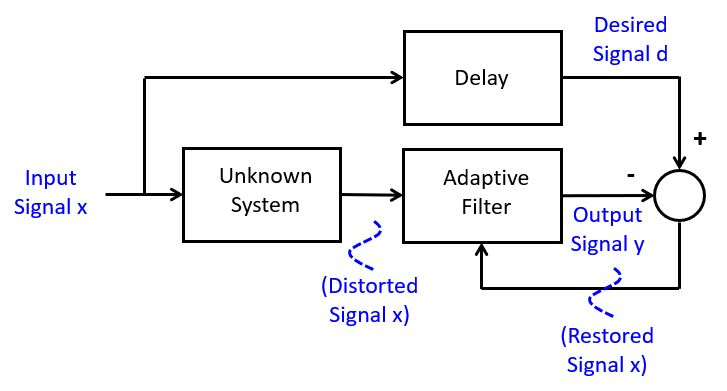
\includegraphics[scale=0.5]{figures/sec2equalization.jpg}
                  \caption{信号矫正滤波器工作过程}
                  \label{fig:equalization}
              \end{figure}
          \end{center}

    \item 自适应预测

          滤波器还可以用于自适应预测一段波形的未来形状。一般而言,自适应滤波器的系数可以用于计算未来波形,在信号编码中可以被使用。
\end{itemize}

自适应滤波器的数学模型如下.

对于第 $n$ 次波形过滤过程,滤波器的滤波参数被定义为$\omega(n)=[\omega_{k}(n)]_0{k=1}^{L}\in\mathbb{R}^{L}$.
初始波形为$x(n)=[x_{k}(n)]_{k=1}^{L}\in\mathbb{R}^{L}$,预期波形为$d(n)=[d_{k}(n)]_{k=1}^{L}\in\mathbb{R}$.

滤波器的输出波形为

\begin{eqnarray*}
    y(n) = x^{T}(n)\omega(n)
\end{eqnarray*}

定义滤波器的单次误差为
\begin{eqnarray*}
    e(n) = y(n)-d(n)
\end{eqnarray*}

并采用最小二乘误差的优化算法进行模型的参数更新训练,即最小化单次误差的 $l_2$ 范数:
\begin{eqnarray*}
    e^2(n) = d^2(n)-2d(n)x^T(n)\omega(n)+\omega^Tx(n)x^T(n)\omega(n)
\end{eqnarray*}

由优化知识结合梯度下降算法我们可以得到最终的参数更新公式如
\begin{equation*}
    \omega(n+1)=\omega(n)+2\beta e(n)x(n),\qquad \tag{B1}
\end{equation*}

\paragraph{\heiti{量化感知技术}}

由于滤波器工作场景硬件设备限制,量化感知技术被用于节约模型训练中的时间空间成本。
量化感知技术主要实现模型实际参数的低精度近似储存。计算机中的参数储存通常由浮点数等相对较高精度的数据格式完成,而相对大型的模型在数据存储时消耗的资源较多。
量化感知技术旨在将原本通过高精度数据格式存储的方式改为用低精度存储参数。
与此同时,量化感知技术希望在训练过程中也采用针对低精度格式的计算方法,相应技术构成了量化感知技术的核心。
\begin{center}
    \begin{figure}[h!]
        \centering
        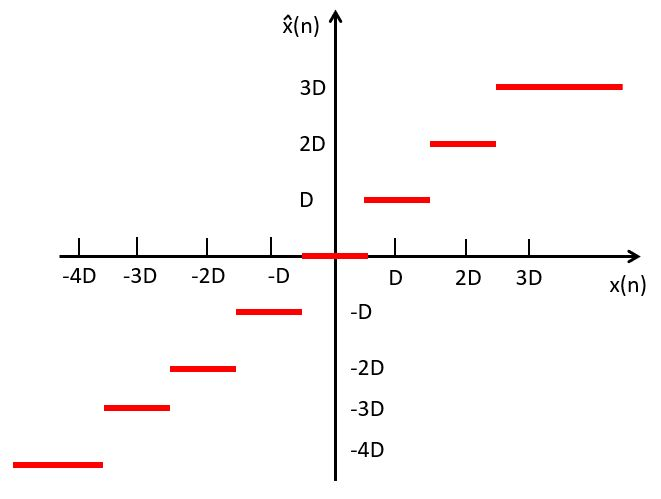
\includegraphics[scale=0.5]{figures/quantizer.jpg}
        \caption{连续型参数的量化离散映射}
        \label{fig:quantizer}
    \end{figure}
\end{center}

当前深度学习框架也增加了许多量化感知方法,这些方法可以在训练过程中直接将参数量化为低精度形式,
并用低精度方法对模型参数进行直接训练。
相对传统的训练方法在训练后将最终参数量化存储而言,前者更为直接地在训练过程中引入量化感知技术,
减少了近似步骤,在精度方面也有提高。

\paragraph{\heiti{自适应量化滤波器}}

自适应滤波器结合量化感知技术是一种提高自适应滤波器模型参数训练效率的方式之一。
将自适应滤波器的模型参数放置于量化感知技术的框架下进行训练,例如搭建量化神经网络还原滤波器结构并搭建相应量化参数的优化算法,最终进行训练。
量化感知技术由于其存储格式上的低精度处理,可以有效地降低存储结构的空间消耗。同时由于量化感知计算的计算复杂度降低,模型进行训练更为快速,即时修正模型参数效率得到提升。

量化感知技术(Quantization Perception)可以减轻神经网络训练上浮点数计算的时间/空间复杂度,从而释放算力进而加速
神经网络的训练。

% 对于浅层神经网络而言采用前向直接估计器 (STE)

% 而使用非前向直接估计器。

% 有关于自适应滤波器 FIR 滤波器

